\chapter{Implementation}

\section{Initial work}
Development was carried out in weekly iterations starting from Monday 27th February 2017. To enable a smooth start to development, several tasks were completed before this, starting with setting up the development and testing environment.

To develop the charades game, both python and OpenCV needed to be set up. Installing python on windows is done by downloading the windows installer from the python.org website and running it - following the instructions on the installation wizard. OpenCV requires the pre-requisites of NumPy (A mathematical library for Python) and SciPy (A scientific library for Python). Both of these were installed using the pip tool (A Package manager for Python). Once these were installed and verified to be working OpenCV was downloaded, extracted and the binary file added to the Python site-packages directory. For more information on setup and running the program, see the README.txt file packaged with the code base.

\section{Iteration 1}
\textbf{Date}: 27/02/2017 \\
\textbf{Features}: 1, 3, 4 \\
\textbf{Overview}: The first iteration focused on putting in place the ground work for the hologram creation application. In addition to developing an understanding for the OpenCV library, tasks for this iteration also included obtaining and displaying a video feed from a web cam, as well as rotating the image obtained from the web cam.

\subsection{OpenCV API}
Due to the diversity of the OpenCV library with regards to its platform deployment and versioning, the documentation for the library is fragmented making examples difficult to find. Most documentation is basic and the online API covers all programming languages. It was for this reason, that much of the first iteration was spent deciphering the way the library should be used. The online documentation did provide a tutorial for the implemention of capturing the output from a web cam \cite{video_capture_tutorial}. This tutorial was used as a starting point for the system (Feature 1).

\subsection{Deep versus shallow copying}
Originally, the feature list contained an additional feature to be implemented during this iteration. The feature was to create 4 copies of the video feed to display them on each side of the pyramid. Original spike work suggested that this could involve creating a deep copy of the VideoCapture output. The reason a deep copy would be required is that each instance of the video feed would need to be rotated independently of the others. If the default operation for copying a video frame in Python is a shallow copy, then both variables will share a pointer to a single object \cite{deep_shallow_copying}. If this is the case, then rotating the video frame will rotate all the instances rather than just one. Through further investigation, it was discovered that each frame of the video was of type NumPy array. Furthermore, the output window, where the video feeds were being displayed, was also a NumPy array. This removes the problem of having to make a deep copy of the array as the numbers from the array can be directly added to the output array rather than copying the frames individually.

\newpage

\section{Iteration 2}
\textbf{Date}: 27/02/2017 \\
\textbf{Features}: 2, 5, 16 \\
\textbf{Overview}: Most work in this iteration involved investigation and implementation of a method for background subtraction in the charades game. This feature was estimated to take 3 or 4 days due to its complexity, as such minor features from the charades game were also added to this iteration.

\subsection{Background subtraction research}
To begin this iteration, research took place to determine the best possible method for background subtraction from the video frame. The "Comparative study of background subtraction algorithms" \cite{background_subtraction_comparison} provided an interesting summary and comparison of possible background subtraction routines. Given the need for real time execution of the background subtraction, it was decided to use the simple background subtraction technique. Simple background subtraction is performed by taking an image of the scene without the subject (foreground) present. For all frames that follow this, the background image is then subtracted from the frame which will leave only the foreground image.

\subsection{Image subtraction}
The simple background subtraction technique was implemented using the first frame captured by the web cam as the background image. Then when displayed, this image was subtracted from the real-time data from the web cam. Originally, this was implemented in full colour but due to the camera shake, auto focus and lighting adjustment made by the camera itself, the background image differed too much from the real-time foreground. To compensate for this, the background images was changed to be grey scale reducing the variance in colour from three channels to one. The grey scale background was then subtracted from a grey scale version of the web cam output and the resulting image was used as a mask. The mask could then be applied to the real-time video feed to only display the content that is outside of the mask. Using a mask improved the quality of the background subtraction, but not to the degree that was acceptable, as the mask that was generated was poor and contained holes due to the quality of the input video.

\subsection{Green screen}
The approach of using a green screen is commonly used in film and television production. This technique involves placing a green screen behind the object of interest, and then removing the green colour from the scene programmatically. The green colour is used for filming humans as it is a stark contrast to most skin tones. This implementation proved more effective in the quality of the output image produced. However, due to the video feed being captured in real-time, the function to remove the background needed fast execution to not reduce the frame rate of the display. The camera being used captured video at a frame rate of 60 frames per second (FPS). Applying the algorithm for removing the background reduced the frame rate to close to 10 FPS as each individual pixel had to be checked to find if the colour was part of the background or foreground. Despite attempts to optimise the algorithm, the best FPS achieved was 15.

The background subtraction algorithm implementation was left at this point to allow for other development to take place during this iteration. Planning allowed for work to continue this during the next iteration providing no set backs were encountered. This was an acceptable decision as a fall-back plan of using a black curtain as the background in the scene could be used if required.

\subsection{Defining the phrases}
Instead of further development on the background subtraction implementation, ideas for possible phrases to be used in the charades game were gathered. This involved research into the types of books and films that are popular with a younger target audience. Most of the phrases were selected from the \textit{"100 best children's books"} list from BookTrust \cite{book_trust} and Sara Schmidt's \textit{"15 Best Kids Movies Of 2016"} publish on screenrant.com \cite{movies_2016}.

Feature 5 was pushed back to the next iteration due to the setbacks with the background subtraction algorithm.

\newpage

\section{Iteration 3}
\textbf{Date}: 06/03/2017 \\
\textbf{Features}: Spike work for Charades Game \\
\textbf{Roll-over features}: 5 \\
\textbf{Overview}: As well as completing the remaining work (Feature 5) from the previous iteration, this iteration covered the set up and spike work for android application development. Whilst in the end the Charades game was implemented as a web application, at this stage of the project, the design was for an android application. This decision will be discussed in more detail in \textbf{Iteration 4}. Finally, this iteration reopened the investigation into the optimisation of the background subtraction algorithm.

\subsection{Android setup}
Android Studio was the IDE chosen for Android development as it is one of the largest Android specific IDEs available. Furthermore, the online documentation for Android Studio provides multiple guides that help with the set up and implementation of a basic android app. After downloading and installing the IDE, the \textit{"Create an Android Project"} guide \cite{create_android_project} was followed to aid in the setup of a blank project. The tutorials that were available meant that spike work was completed quickly and yielded a basic prototype for the android application.

\subsection{Android status bar}


\begin{figure}[h!]
	\centering{
		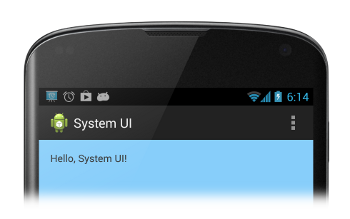
\includegraphics[scale=0.9]{Chapter3/status_bar_show.png}
		\caption{Shows a mock android application with the status bar open. The status bar is the black panel with the text "System UI" and the approve device information such as notification, signal, battery, ect. This image was taken from the "Hiding the Status Bar" tutorial created by the Android development team \cite{hide_status_bar}.}
		\label{fig:status_bar}
	}
\end{figure}


An additional task that was required alongside the creation of the welcome screen of the Android app was to remove the status bar from the Graphical User Interface (GUI). The status bar can be seen in Figure \ref{fig:status_bar} and the \textit{"Hiding the Status Bar"} tutorial \cite{hide_status_bar} from the Android developer site, gave an insight into how this could be removed from the app. When implementing the suggested changes from the tutorial, an error occurred routing from the call to the getActionBar() method that returns a pointer to the status bar. A stack overflow issue detailing this error \cite{sof_status_bar_err}, helped to diagnose the cause of the issue. The version of android being used was utilising the new
\begin{verbatim}
android.support.v7.app.ActionBarActivity
\end{verbatim}
which needed to be accessed as a support status bar rather than the older style regular status bar. This could be done using the function: 
\begin{verbatim}
getSupportActionBar()
\end{verbatim}

\subsection{UI testing}
To ensure that all elements of the Android application were subject to some form of automated testing, UI tests were developed for the Android app. These tests included checking page contents as well as page transitions to ensure that the expected content was visible and the buttons functioned correctly. As described in the Android developers guide \textit{"Testing Apps on Android"} \cite{testing_apps_on_android}, two types of test are commonly used for testing Android applications.

\begin{itemize}
	\item \textbf{Local unit tests}: Unit tests in this case are similar to any standard unit test for a normal code base. They test function input and output given various states. These tests are run on the local machine using the Java Virtual Machine (JVM) and have access to the Android specific API functions.
	
	\item \textbf{Instrumented tests}: By contrast, the Instrumented tests run on a hardware device or emulator. They are designed to test the app while it is running rather than testing individual functions, like a unit test. This allows for tests that exercise button transitions or page content to be run in an automated way.
\end{itemize}

For the UI testing, Instrumentation tests were developed and run on a mobile device attached to the development machine.

Whilst running tests for page content was straightforward, attempting to test page transitions proved more complex. A stack overflow issue was found that helped in to determine how this operation could be achieved \cite{sof_android_button_test}. The answer to the issue detailed using an ActivityMonitor class to listen for an Android Intent (the commands issued at the time of page transition) being executed.


\subsection{Background subtraction multi-threading}
Finally, this iteration revisited the background subtraction algorithm. Having already implemented the green screen algorithm, the algorithm or execution of the algorithm needed to be optimised to produce an acceptable frame rate. To do this, investigation in Python multi-threading took place. Each pixel in the input image needed to be checked and if it was above a certain value of green, changed to be black. This operation was performed on every pixel independently one after another. To improve the speed of execution, instead of checking the full array of the image in the main thread, the image was divided into 4 quadrants and each processed in a separate thread. Initially this was done in place in the array where each thread was given a start and end index to check. However, after implementing this solution, it was found to not have decreased the execution speed. This was the result of the array being locked while processing. To avoid multiple threads accessing the same NumPy array and potential corrupting the data, the array is locked while one thread accesses it meaning that the next thread must wait for the first to finish. 

By creating new array objects that relate to each quadrant the lock problem was avoided, however only a slight decrease in execution time was found. More detailed investigation revealed that this was caused by the time taken to initialise new arrays with the data from each quadrant.

Again, as no solution was found for execution time issue, development of the background subtraction algorithm was halted. Instead it was decided to use a black background when filming. Whilst this solution offers less versatility in the location where actors can be filmed, it means that the frame rate of the hologram remains close to that of the camera feed. 

  
\newpage

\section{Iteration 4}
\textbf{Date}: 13/03/2017 \\
\textbf{Features}: 6, 7, 8 \\
\textbf{Overview}: Aberystwyth University Science Week was scheduled to begin on the 14th March 2017 and last a duration of three days. All the work required for the prototype (Feature 1-4) had been completed or alternative solutions found, as such it was possible to take the prototype to the event to test it with the target audience. In addition, this iteration concluded with a demonstration of the project so far on Friday 17th March. 

\subsection{Aberystwyth Science Week 2017}

\begin{figure}[h!]
	\centering{
		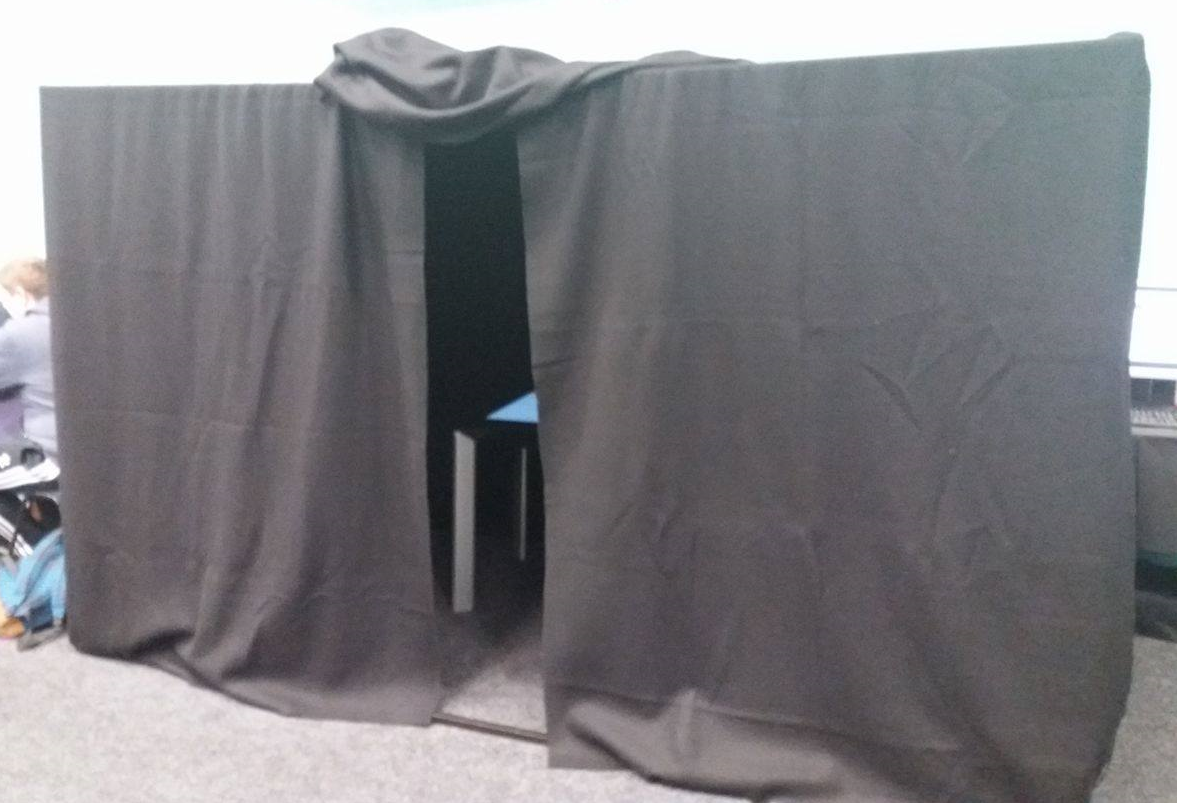
\includegraphics[scale=0.3]{Chapter3/viewing_area_science_week.png}
		\caption{Shows the viewing area for the real-time hologram creation system at the Aberystwyth University Science Week 2017. Inside, part of the touch screen table (being used as the display monitor for the system) is visible.}
		\label{fig:science_week_viewing_area}
	}
\end{figure}


The entities listed in the component diagram (the staging area, viewing area and image processing machine) were all constructed at the event venue. Figure \ref{fig:science_week_viewing_area} shows the viewing area (large black tent housing the monitor for the Pepper's Ghost Pyramid). To the right of the tent a camera attached to a computer was set up to record members of the audience. The camera was attached to the computer via a USB cable and the computer was attached to the external monitor in the tent via a HDMI cable.

Two main pieces of feedback could be inferred from using the prototype at the event. The first is that it proved a great success, with the clear majority of visiting students appearing greatly interested and engaged by the impactful display. The second was that students were not given much time at the event (most schools were present for an hour), meaning that the time that students were able to spend at each stall was limited. Originally, the Charades Game was designed to be played where actors and viewers would swap every time a correct answer was given, as would be the rules in a conventional game of charades. However, after discovering the limited time window for each activity at the science week, this concept was adjusted going forward to better suit the use case. To do this, two changes to the game rules were made:

\begin{itemize}
	 \item Actors act three phrases, and a points system was used, giving viewers points for correct guesses. At the end of each round, the viewer with the highest points would become the actor. This change enabled more time to be spent using the system, and less time for the member of the audience to be swapping roles.
	 
	 \item The subject of the phrase was changed to make more phrases single words and, rather than using conventional genres such as books and films, genres were changed to be activities and animals. These new genres meant a large amount of phrases were shorter and avoided long titles with simple words. A good example of where long titles would have been a problem is with the book "The Lion, the witch and the wardrobe". This phrase could take some time to act out fully due to the large number of words and it is also difficult to act simple words like "The".
\end{itemize} 

\subsection{Mid project demonstration and conclusions}
The mid project demonstration overall was a success and the demonstration of the software worked well. However, the question was raised as to why the charades system had been designed as an android application. The original reasoning for an android app was to promote the use of hand held devices for interaction with the system. Moreover, an Android app can potentially remove the reliance on the internet via the use of Bluetooth or locally connecting the devices together. This is an important factor to consider if, for example, an outreach event was being held in an area or building with poor reception. Furthermore, an android application removes problems that can occur with users attempting to manipulate the system via the URL which can be the case in some web apps.

Despite this, on re-evaluation of the project requirements and the final use case of the system, a web app was a better choice. The web app implementation removes many of the complications that could be faced with an android application which include:
\begin{itemize}
	\item Enabling devices to communicate with one another: Whilst there are many technologies for performing communications between android applications such as over the internet, via Bluetooth or through a peer-to-peer system, these technologies can be difficult to implement and test.
	\item Limiting the number of devices that are available: Whilst the event organisers would normally be able to get several tablets and mobile devices to use with the system. If users wished to join in on their own devices this would require that both the device they are using is on the android operating system, and the app is available on the Google Play Store.
\end{itemize}

A web app solves the above problems as it is already hosted on the internet which will allow for implicit communication between device accessing the system. Furthermore, the web app will be platform independent as the system code is executed server side and users interact with it through a web client.

This decision was difficult as due to the events of the week, little progress had been made on the android application. Starting again with a web application would mean further setbacks, but at the time the decision was made that it would lead to a better product.

\newpage

\section{Iteration 5}
\textbf{Date}: 20/03/2017 \\
\textbf{Features}: 9, 10 \\
\textbf{Roll-over features}: 5, 6, 7, 8 \\
\textbf{Overview}: This iteration's first task was to adjust the features list schedule due to the decision to change to a web app from an Android app. Therefore, this iteration dealt with the roll over issues from the previous iterations, and Feature 9 and 10 (which were originally planned for this iteration) were redistributed among future iterations.

\subsection{Django}
As the hologram creation software already used the Python programming language, it was logical to use a Python framework for implementation of the website. Several Python web framework exist with the most popular being Django, Flask and Pyramid. The article \textit{"Django vs Flask vs Pyramid: Choosing a Python Web Framework"} written by Ryan Brown \cite{python_webframework_comparison}, was a useful resource in making a decision regarding the best framework to use. In the Article, Django is identified as the most popular of the three as well as being best suited to mid scale projects like the Charades system. Furthermore, Django uses many familiar keywords and concepts to those ruby on rails which is a technology that the developer had used prior. Finally, an excellent tutorial for the Django web framework by Nigel George, \textit{"Masting Django: Core"} \cite{django_book} is available for free online. 

\subsection{Model}
As described in \textit{"Mastering Django: Core} \cite{django_book}, the initial web site setup was fast and straightforward. This process was made simpler by not having any requirement for a database and having models written as Python classes. However, using Python class meant that there was an additional requirement for tests to ensure the model functioned correctly. This would not have been required of a database as they are tested by the database supplier (for example SQL) before release. The tests for the Python class models were written as Python unit tests. As the model did not rely on the Django web framework, classes could be considered independent from the rest of the system and tested in isolation.

The model can be found in the directory /charades/charades/ directory. The model consists of actor.py, game.py, viewer.py phrases.py and strings.py.

\subsection{Template}
The templates in Django are written in html and can use embedded Python code to execute additional commands or access variables. The variables are pushed to the template through the controller and can then be accessed by surrounding them in double curly brackets:
\begin{verbatim}
{{ variable_name }}
\end{verbatim}

Embedding python code also proved powerful for flow control and conditional statements. An example of both of these being used can be found in Appendix C section \textit{Embedded Python}.

The template code can be found in the /charades/templates directory.

\subsection{View}
The view code is the controller for the website and acts as the link between the model (data) and the template (information displayed to the client). The views.py file is where this code is stored and consists of multiple view functions. The view functions must have take an input parameter of type request (which is a HTTP request header) and must return a request along with some rendered data (the template code). It is at the point where the request is returned that additional data can be provided to the template in the form of a python dictionary.

The HTTP request is handled by the urls.py file which holds the routing information between the URL and the controller. Figure \ref{fig:django_routing} visually represents how these interactions take place.

The view code can be found in the /charades/charades/views.py file.

\begin{figure}[h!]
	\centering{
		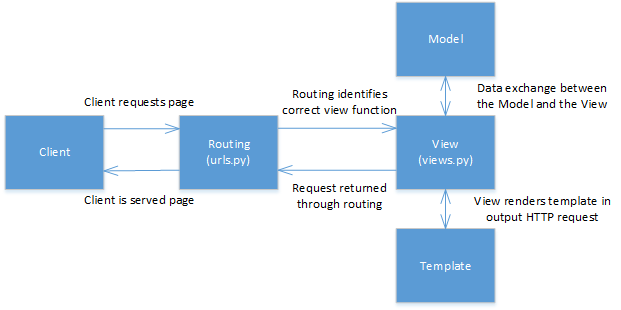
\includegraphics[scale=0.9]{Chapter3/django_routing.png}
		\caption{Show the interactions between the client, the urls.py (routing) file, the template, the view and the model in the Django web framework.}
		\label{fig:django_routing}
	}
\end{figure}

\newpage

\section{Iteration 6}
\textbf{Date}: 27/03/2017 \\
\textbf{Features}: 9, 10, 11 \\
\textbf{Overview}: This iteration covered access and security for the Charades Game and dealt with functions to ensure that only those at an event would be able to log on. Furthermore, to improve the security of malicious users, redirects were put in place to stop access to certain pages depending on the game state.

\subsection{Session password}
To disable access from those outside an event (such as the Aberystwyth Science Week), a session password was added to the landing page of the website. When a user chooses a type (actor or viewer), they are also required to provide the session password to access the system. By default, the session password is stored in the view code as \textit{"BSW18"} but this can be changed easily. If mobile devices capable of accessing the system were provided for an event where the system was in use, the organisers would be able to type in the session password before the arrival of any visitors. Alternatively, (if guests were to use their own devices) the session password could be displayed on a sign near the viewing area enabling users to log in themselves.

\subsection{Cookies}
When a valid session password has been provided, the password is then stored client side in a cookie. The Django online documentation \cite{django_cookies} provided a tutorial which aided greatly in the implementation of a session cookie. In addition, the cookie also stores the type of user (actor or viewer) and, if the user is a viewer, the unique number used to identify them. This unique number is called the viewer\_number and is generated by the system when a new viewer joins. The number can then be used to lookup the viewers score:

\begin{verbatim}
	viewer_number = request.session['viewer_number']
	...
	viewer = GAME.lookup_viewer(viewer_number)
	points = viewer.points
\end{verbatim}

The above code is from the waiting\_for\_actor function in the \/charades\/charades\/views.py file. The code returns the current score of the viewer accessing the waiting\_for\_actor.html page. The code first finds the viewer number from the session variable (cookie), and then calls the lookup\_viewer function in the Game class, using the viewer\_number as input. This will return the Viewer object relating to the viewer\_number provided. Finally this object can be used to see how many points the user has accumulated.

\subsection{Redirects}
\subsubsection{State based redirects}
Each page of the website (excluding the landing page) queries a part of the model. It is possible that, without proper handling, either intentionally or not, a user can access a page that the system state does not yet access to as it is missing data required to render the page. An example of this is if a viewer attempted to access the guess.html page (where they are asked to guess the current word or phrase) before the actor has chosen a phrase. Accessing this page at this time could cause errors to be thrown and potentially corrupt the game state. To stop this from happening, state based redirects have been added to the website controller. These are functions that, instead of returning the page content that would normally be provided from the requested URL, redirect the user to a different URL. The different URL will then handle the request appropriately. In the above case of accessing the guess.html page before it is ready, the viewer will be redirected to the instructions page which displays a "Please wait" message as shown in Figure \ref{fig:state_redirect}.

\begin{figure}[h!]
	\centering{
		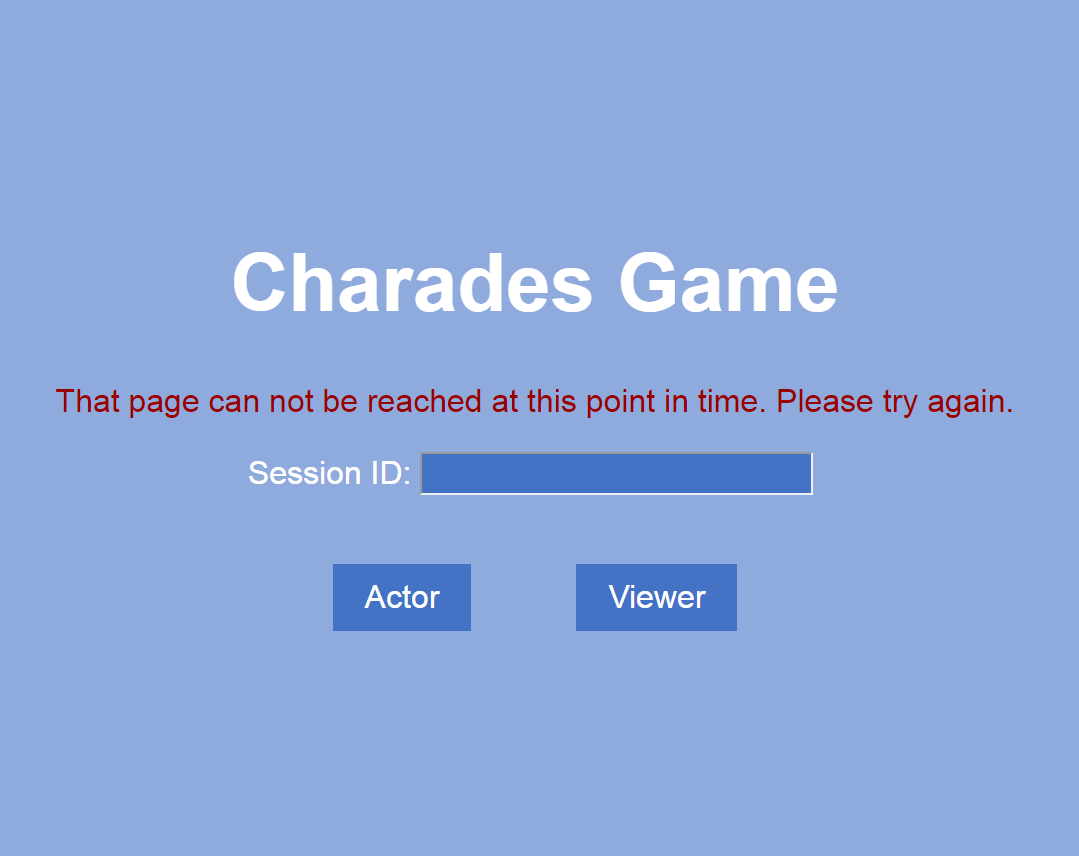
\includegraphics[scale=0.45]{Chapter3/state_redirect.png}
		\caption{Shows the outcome of a state based redirect in the Charades Game.}
		\label{fig:state_redirect}
	}
\end{figure}
\newpage

\subsubsection{User type redirects}
Similarly, users can attempt to access webpages that are only designed for a different type of user. An example of this is that the phrase\_selection.html page is designed for the actor to select a phrase to be acted. Once selected this data is then passed to the model and the viewers are able to guess the word or phrase. It should not be possible for a viewer to access the select\_phrase.html at any time, therefore user type redirects have been added to the controller to ensure this is not possible. The user type redirects are designed to check the type of user attempting to access the content by searching for the 'user\_type' entry in the session variable. If the incorrect user\_type, or no user\_type at all, is found in the session variable, the client will be redirected to the landing page, and an error message will be displayed as shown in Figure \ref{fig:user_type_redirect}.

\begin{figure}[h!]
	\centering{
		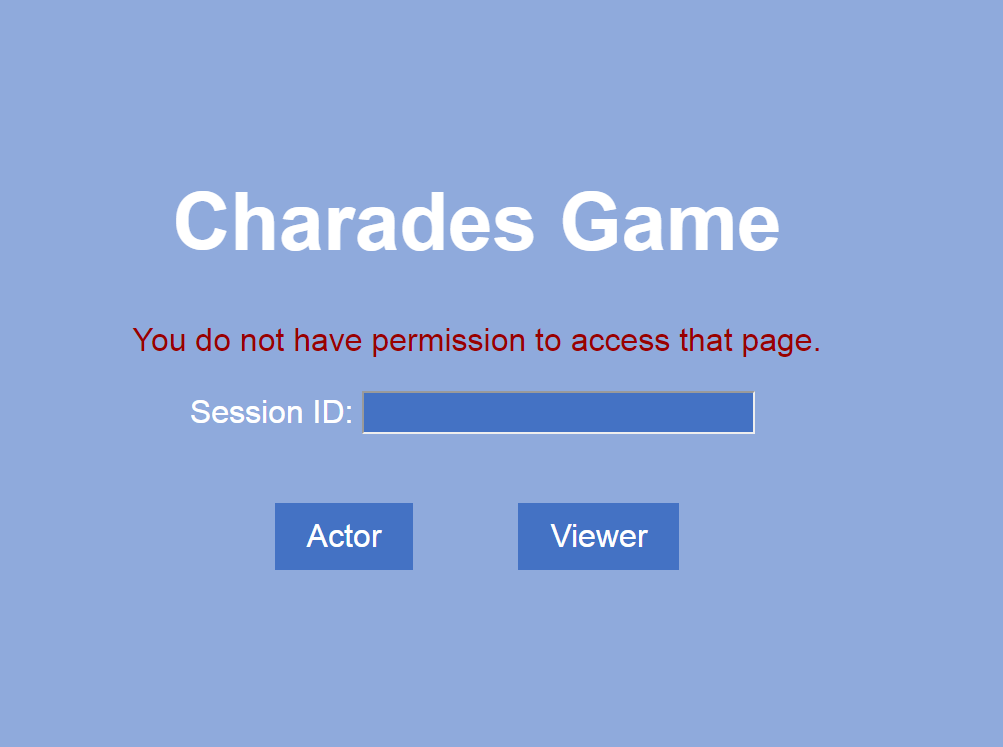
\includegraphics[scale=0.45]{Chapter3/user_type_redirect.png}
		\caption{Shows the outcome of a user type redirect in the Charades Game.}
		\label{fig:user_type_redirect}
	}
\end{figure}

\newpage

\section{Iteration 7}
\textbf{Date}: 03/04/2017 \\
\textbf{Features}: 12, 13, 14 \\
\textbf{Overview}: This iteration focused on allowing communication between user in real (or near to real) time. As well as implementing a solution to this, several other possible solutions were investigated and evaluated. 

\subsection{Real time updates}
The charades game has multiple users logged in at the same time and has several scenarios where interactions need to take place in real-time. An example of a real time interaction, is that when a phrase is guessed correctly by a viewer, the actor must be informed and prompted to select a different word.

When the Django framework was created, it was designed to handle static website that were more common of those seen 5 or 10 years ago. In this respect, at its core Django is built around answering requests from the client, but does not have any methods to push data to the client by default. However, many technologies provide solutions to real time communications for the web and can be implemented in Django. The approach chosen for this project was to use an API and a polling system to mimic the pushing of data from the server side to the client. 

An alternative consideration was made to use the new Django Channels technology. Django Channels provide a way to opening a bi-directional connection between the server and the client, allowing data to be pushed both ways (client to server and server to client)\cite{django_channels}. This technology utilises the new WebSocket protocol. Whilst this technology would provide a solution to the aforementioned problem, implementing the technology is a more complex task than a implementing a polling system. It is however a better and more long term solution but, the additional time it would have taken to implement would have set the project back further.

\subsection{API}
An Application Programming Interface (API) was created as a way to programmatically assess the current state of the system. As with any Django page, when a request is sent from a client (for example the user types the page URL into the address bar) the page is loaded and any data that is embedded in the template will be updated automatically. In the case of an API, simple data that represents a fact in the system can be displayed. In the case of phrase\_ready.html, this page, when loaded, is given data from the controller. The controller function (See Appendix C, Section \textit{phrase\_ready API}) checks the current state of the system, and produces a True or False value as to whether the phrase is in a guessable state. The state of the system will change depending on the user interaction with the system. For example, if a phrase has not yet been selected by the actor, the phrase\_ready API will display False. Once a phrase has been selected, the controller will receive the data from the client request, update the current phrase in the system and then, when the API is polled (loaded) it will have the new value of True.

\subsection{Polling}
As Django does not provide a built in methods of pushing data to the client (as discussed above), the client most poll the API to establish if the state of the system has changed. This is done using the JavaScript setInterval() function \cite{js_setinterval}. This function takes a parameter of another function and a time interval given in milliseconds. When that number of milliseconds has passed, the provided function will be executed. To poll the API the project used a function that was designed to retrieve information from the API pages using an HTTP GET request. This function (detailed in Appendix C, section \textit{Polling function}) was the primary input to the set interval function. When the data is received from the API, conditional statements within the function decide what should happen. In most cases this is a page refresh and then the controller will supply new data to the page.

Depending on the polling function, the API is normally polled every second with some cases having larger polling intervals if  an instantaneous answer is not required. This method of communication does have one small caveat, if two users were to guess the word within one second of each other, it is possible that both viewers would receive points. The reason for this interaction is that when a viewer guesses a phrase correctly, the API is updated and then all the viewers (on the guess.html page) are redirected to the waiting\_for\_actor.html page. During the time the other viewers are polling the API it is possible that a guess could still be submitted and, if correct, the controller would increment the score of the viewer who guessed correctly. This would result in the above interaction where two or more player potentially score points if they guess within a second of each other. Statistically, a full second window for another viewer to guess is the worst case scenario as it is likely that a viewer makes a correct guess mid way through a polling cycle. This would result in a 0.5 second window which was deemed acceptable.

\newpage

\section{Iteration 8}
\textbf{Date}: 10/04/2017 \\
\textbf{Features}: 15, 17 \\
\textbf{Overview}: The final iteration covered two main tasks. The first was to decide on a end game condition and scoring, and the second to perform some refactoring of the of the Charades Game to improve readability and maintainability.

\subsection{End game conditions and scoring}
To ensure that the game was completed in a timely manor and the outcome was fair the scoring system and rules had to be decided upon. The rules, as previously mentioned were changed to include a scoring system as well as multiple rounds. The game lasts for a duration of three rounds, where a round is a single phrase being guessed. Although the main purpose of the game is to be an aid to showcase the hologram system, for the younger target audience, having a friendly competition would prove more interesting for them. The phrase dictionary consists of one or two word phrases, as such the whole phrase is worth 20 points, and a single word is worth 10. At the end of a round a new actor is chosen based on either a volunteer or the highest scoring viewer.

\subsection{Refactoring}
The controller (views.py) for the Charades Game had been continually added to throughout the development period. It contained all the functions for executing control code in a single file, and had some code duplication. To improve this, the code was refactored to firstly ensure that duplicated code was removed and secondly to make the controller easy to read. This was an important step as, providing this system would be used in the future, it would most likely require adaptation to remain current. Refactoring the code base also gave the advantage of allowing more tests to be added to the simpler helper functions which improved the overall test coverage of the system.

\newpage

\section{Implementation review}
The major objectives set out at the beginning of the project have all been met with varying degrees of success. Whilst the main objectives regarding the actual system use cases itself have all been met, some of the other areas of the system could be improved relative to the criteria of the objectives. 

The system should have been designed with a greater focus on the ease of use in mind. Whilst not tested explicitly on the target audience, with more effort put in to UI design, the system could have been easier to use. As a direct result of this, there is an instructions page for both sets of users built into the system, however, if the web app requires written instructions, then it could be argued that the system could be simplified.

Whilst the hologram system is thoroughly tested, there could be room for additional automated testing of the Charades Game. The view (controller) could be tested in an automated way rather than the manual testing it underwent.

However, the rest of the objectives have been met well, especially given the large setback in the middle of the project regarding the change from android app to web app.